\documentclass{article}
\usepackage[margin=1in]{geometry}
\usepackage[final]{microtype}
\usepackage{amsmath}
\usepackage{amssymb}
\usepackage{graphicx}
\usepackage{enumitem}

\title{AMAT 491 Assignment 4}
\date{Dec 11 2017}
\author{Ian McKenzie}

\begin{document}
\pagenumbering{gobble}
\maketitle
\newpage
\pagenumbering{arabic}

% Question 1
\section{}
\subsection*{a.}
Let a be an nxn tridiagonal matrix. Let a be the diagonal, b be the
subdiagonal, and c be the superdiagonal. Then to find l, u, and d such
that l is the subdiagonal of a lower matrix; and u and d are the
superdiagonal and diagonal of the upper matrix such that \(L*U=A\) we
follow the following algorithm.
\begin{enumerate}[label*=\arabic*.]
  \item First, prepend a 0 to the b vector and append a 0 to the c
    vector so that all vectors are of length n.
  \item Set u = c.
  \item Set the first element of d equal to the first element of a.
  \item For each k from 2 to n,
    \begin{enumerate}[label*=\arabic*.]
    \item Set \(l(k) = b(k)/d(k-1)\)
    \item Set \(d(k) = a(k) - l(k)\cdot c(k-1)\)
    \end{enumerate}
  \item Remove the first element of l and the last element of u.
\end{enumerate}
\subsection*{b.}
See \texttt{TriLU.m} and \texttt{queston1.m}.

% Question 2
\section{}
See \texttt{myJacobi.m}, \texttt{myGaussSeidel.m},
\texttt{relative\_error.m}, and \texttt{question2.m}.

% Question 3
\section{}
Let's start from the definition of a matrix norm
\[|||A||| = \underset{\substack{x\epsilon\mathbb{R}\\ x\neq0}}{\max}
\frac{||Ax||}{||x||}\]
When we specify that we are looking for the infinity-norm, this leaves
us with
\begin{align*}
  |||A|||_{\infty} &= \underset{\substack{x\epsilon\mathbb{R}\\ x\neq0}}{\max}
  \frac{||Ax||_{\infty}}{||x||_{\infty}}\\
  &= \frac{\underset{1\leq i \leq n}{\max}\left|\sum\limits^n_{j=1}a_{ij}x_j\right|}
       {\underset{1\leq i \leq n}{\max} \left|x_j\right|}\\
  &= \frac{\underset{1\leq i \leq n}{\max}\sum\limits^n_{j=1}\left|a_{ij}\right|\left|x_j\right|}
       {\underset{1\leq i \leq n}{\max} \left|x_j\right|}\\
  &= \frac{\underset{1\leq i \leq n}{\max} \left|x_j\right|\underset{1\leq i \leq n}{\max}\sum\limits^n_{j=1}\left|a_{ij}\right|}
       {\underset{1\leq i \leq n}{\max} \left|x_j\right|}\\
  &= \underset{1\leq i \leq n}{\max}\sum\limits^n_{j=1}\left|a_{ij}\right|
\end{align*}

% Question 4
\section{}
\subsection{}
\subsubsection{}
For the Jacobi Method we have
\[B_j = (I-D^{-1}A) =
\begin{bmatrix}
  0  &  1/2  &  -1/2\\
  -1 &   0   &   -1\\
  1/2&  1/2  &    0
\end{bmatrix}
\]
and for the Gauss-Seidel Method we have
\[B_{GS} = (I-L^{-1}A) =
\begin{bmatrix}
  0  &  1/2  & -1/2\\
  0  & -1/2  & -1/2\\
  0  &   0   & -1/2
\end{bmatrix}
\]
\subsubsection{}
For the Jacobi matrix we have
\[\rho(B_J)
= max\left(abs\left(\left\{0,\frac{\sqrt{5}}{2}i,\frac{-\sqrt{5}}{2}i\right\}\right)\right)
= \frac{\sqrt{5}}{2}\]
and for the Gauss-Seidel matrix we have
\[\rho(B_{GS})
= max\left(abs\left(\left\{0,\frac{-1}{2},\frac{-1}{2}\right\}\right)\right)
= \frac{1}{2}\]
\subsubsection{}
After 25 iterations, the Jacobi method finds the solution of
\([-20.8279,2,-22.8279]'\). Even after many more iterations, it fails
to converge to the correct solution.\\
On the other had, the Gauss-Seidel method converges quickly, and the
relative error rapidly decreases.
\begin{center}
  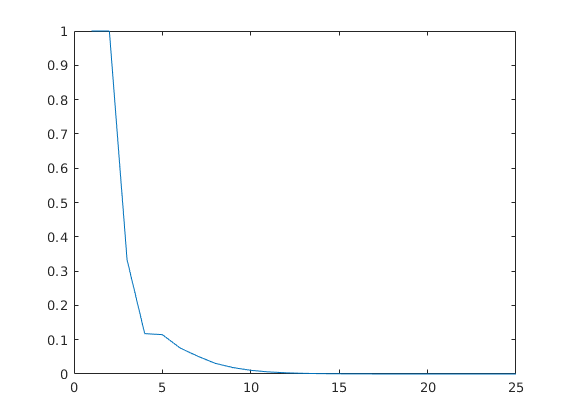
\includegraphics[width=0.4\textwidth]{figures/Question4/Part1/GaussSeidelConvergence}
\end{center}
These results are expected because of the size of the spectral radius.

\subsection{}
\subsubsection{}
For the Jacobi Method we have
\[B_j = (I-D^{-1}A) =
\begin{bmatrix}
   0 & -2  & 2\\
  -1 &  0  &-1\\
  -2 & -2  & 0
\end{bmatrix}
\]
and for the Gauss-Seidel Method we have
\[B_{GS} = (I-L^{-1}A) =
\begin{bmatrix}
  0 & -2 & 2\\
  0 &  2 &-3\\
  0 &  0 & 2
\end{bmatrix}
\]
\subsubsection{}
For the Jacobi matrix we have 
\[\rho(B_J)
= max\left(abs\left(\left\{0,0,0\right\}\right)\right)
= 0\]
and for the Gauss-Seidel matrix we have
\[\rho(B_{GS})
= max\left(abs\left(\left\{0,2,2\right\}\right)\right)
= 2\]
\subsubsection{}
After only four iterations, the Jacobi method converges to the correct
answer.\\ For the Gauss-Seidel method, it results in a very incorrect
answer, and with increasing iterations the result gets worse. \\ Again
these results are expected because of the size of the spectral radius.

% Question 5
\section{}
First we begin with the definitions \(Ax=b\) and \(\tilde{A}\tilde{x}
= \tilde{b}\). From that we can see
\begin{align*}
  A\tilde{x} &= \tilde{b} - (\tilde{A} - A)\tilde{x}\\
  A\tilde{x} - Ax &= \tilde{b} - b - (\tilde{A} - A)\tilde{x}\\
  A^{-1}A(\tilde{x} - x) &= A^{-1}(\tilde{b}-b(\tilde{A}-A)\tilde{x})\\
\end{align*}
And taking the norm of both sides we find
\begin{align*}
  ||\tilde{x} - x|| &= ||A^{-1}(\tilde{b} - b - (\tilde{A} - A)\tilde{x})||\\
  &\leq |||A^{-1}|||\cdot||(\tilde{b} - b - (\tilde{A} - A)\tilde{x}||)\\
  &\leq |||A^{-1}|||\cdot(||\tilde{b} - b|| + ||-1*(\tilde{A} - A)||\cdot||\tilde{x}||)\\
  &\leq |||A^{-1}|||\cdot|||\tilde{A} - A|||\cdot||\tilde{x} - x||
      + |||A^{-1}|||\cdot(||\tilde{b} - b|| + |||\tilde{A} - A|||\cdot||x||)
\end{align*}
And by rearranging, we see
\begin{align*}
  (1-|||A^{-1}|||\cdot|||\tilde{A}-A|||)\frac{||\tilde{x}-x||}{||x||}
  &\leq |||A^{-1}|||\left(\frac{||\tilde{b}-b||}{||x||} + |||\tilde{A}-A|||\right)\\
  \left(1-|||A^{-1}|||\cdot|||A|||\frac{|||\tilde{A}-A|||}{|||A|||}\right)
  &\leq |||A^{-1}|||\cdot|||A||| \left(\frac{||\tilde{b}-b||}{||b||} +
  \frac{|||\tilde{A}-A|||}{|||A|||}\right)
\end{align*}
And finally we find
\[
\frac{||\tilde{x}-x||}{||x||} \leq
\frac{cond(A)}{1-|||A^{-1}|||\cdot|||\tilde{A}-A|||}
\left(\frac{||\tilde{b}-b||}{||b||} + \frac{|||A-\tilde{A}|||}{|||A|||}\right)
\]

\end{document}
